\chapter{Virasoro 代数的张量网络实现}
\label{chap:virasoro}

临界格点模型是研究\emph{共形场论} (conformal field theory, CFT) 的有力工具。有许多格点模型能够揭示出重要的 CFT 数据,而其中最基本也是最重要的一类称为\emph{最小模型} (minimal models)。它们同时也是严格可解模型,而对应的拓扑以及范畴对称性可以通过\emph{融合范畴}添加进来\cite{vanhove2018mapping,aasen2020topological,huang2022numerical,vanhove2022critical}。

这些经典格点模型的配分函数通常可以表示为张量网络的形式。利用 TRG 和 TNR 等重整化算法\cite{levin2007tensor,evenbly2015tensor1},可以通过控制连接维数来得到任意精度的不动点张量,从而可以高效地获取基态以及较低能级激发态(即“后代”)的对应数据。因此,这套方案有望能为分类 CFT 提供了一种数值的角度。

刻画二维 CFT 的一个重要特性是\emph{Virasoro 对称性} (Virasoro symmetry) 以及更一般情况下的\emph{Kac--Moody 对称性} (Kac--Moody symmetry),在格点模型中已有很多工作给出了它们的实现\cite{pasquier1990common,koo1994representations,milsted2017extraction,zou2018conformal,hongler2022conformal,wang2022emergence}。这些方案主要集中于构造一些作用在一维格点 Hilbert 空间上的离散算符,并对其参数取一些各向异性的极限。然而,对于一般的张量网络表示,特别是通过重整化算法得到的不动点张量,其元素往往都是数值的,没有可供展开的参数。因此使用这些方法将难以构造 Virasoro 和 Kac--Moody 生成元。

在本章中,我们将介绍一种构造 Virasoro 代数以及 Kac--Moody 代数的新方案\cite{wang2022virasoro,zeng2023virasoro}。注意到 CFT 中的初级场及其后代可以从圆柱形的配分函数张量网络中提取出来\cite{hauru2016topological},而其中能动量张量以及流算符则与 Virasoro 和 Kac--Moody 代数相关联。具体来说,我们借用了\emph{离散全纯性} (discrete holomorphicity)\cite{cardy2009discrete}的概念,将代数生成元定义中的积分用一个新的圆柱形张量网络来表示,并把的能动量张量(或流算符)插入其中。由此得到的 Virasoro 和 Kac--Moody 生成元可以作用在任意的本征态上,进而可以用来检验这一方法的有效性。

对于\emph{有限尺寸效应} (finite size effect) 影响更为显著的系统(例如一些弦网模型的配分函数,见 \ref{sec:strange-correlator} 节),即使是采用尺寸相对较大的圆柱,也很难从中得到准确的 CFT 能谱等数据。为此,我们首先对不同大小的圆柱进行精确对角化,并根据拟合结果来区分不同的本征态;对于混淆较为严重的态,我们还使用\emph{拓扑投影算符} (topological projectors)\cite{bultinck2017anyons,williamson2017symmetry,aasen2020topological}将转移矩阵投影到对应于特定拓扑荷的子空间中。这样最终能够获得符合预期精度的能动量张量以及对应的 Virasoro 生成元。

\section{二维共形场论回顾}

\emph{共形场论} (conformal field theory, CFT)\cite{belavin1984infinite,ginsparg1988applied,francesco2012conformal} 的诞生源于对相变与临界现象的研究。在(二阶)相变点附近,系统应当具有\emph{标度不变性} (scaling invariance);而在二维情况下,标度不变性与共形不变性是等价的。这就意味着可以用满足\emph{共形对称性} (conformal symmetry) 的量子场论——即共形场论——来处理临界系统。

\subsection{共形对称性与能动量张量}

二维 CFT 可以用复平面上的坐标 $z$ 和 $\bar{z}$ 来描述。根据 Cauchy--Riemann 条件,共形变换 $z\to w(z)$ 和 $\bar{z}\to\bar{w}(\bar{z})$ 分别是\emph{全纯} (holomorphic) 和\emph{反全纯} (anti-holomorphic) 的,即它们只是 $z$ 和 $\bar{z}$ 的函数。在这一共形变换下,满足
\begin{equation}
  \phi(z,\bar{z}) \to \phi'(w,\bar{w}) =
  \left( \dv{w}{z} \right)^{-h} \left( \dv{\bar{w}}{\bar{z}} \right)^{-\bar{h}} \phi(z,\bar{z})
  \label{eq:quasi-primary-field}
\end{equation}
变换关系的场 $\phi$ 称为\emph{准初级场} (quasi-primary field),其中
\begin{equation}
  h = \frac12 \bigl( \Delta+s \bigr), \quad \bar{h} = \frac12 \bigl( \Delta-s \bigr)
\end{equation}
称为\emph{共形维数} (conformal dimension),而 $\Delta$ 和 $s$ 分别称为\emph{标度维数} (scaling dimension) 和\emph{自旋} (spin),它们反映了 $\phi$ 在标度和旋转变换下的性质。如果对任意的局部共形变换,式~\eqref{eq:quasi-primary-field} 都成立,则称 $\phi$ 为\emph{初级场} (primary field)。

根据 Noether 定理,(连续)对称性会与某种守恒流相对应。因而我们可以为一个一般的局部坐标变换定义\emph{能动量张量} (energy-momentum tensor),也称\emph{应力张量} (stress tensor)。在共形对称性的条件下,能动量张量 $T^{\mu\nu}$ 可以取为对称且无迹的,即只保留 $T(z)\coloneq T_{zz}(z)$ 和 $\bar{T}(\bar{z})\coloneq T_{\bar{z}\bar{z}}(\bar{z})$,同时它们也是(反)全纯函数\cite{ginsparg1988applied,cardy2010conformal,francesco2012conformal}。$T$ 和 $\bar{T}$ 的共形维数分别为 $(h_T,\bar{h}_T)=(2,0)$ 和 $(h_{\bar{T}},\bar{h}_{\bar{T}})=(0,2)$,即
\begin{equation}
  \Delta_T = \Delta_{\bar{T}} = 2, \quad s_T = 2, \quad s_{\bar{T}} = -2.
\end{equation}

对于共形维数为 $(h,\bar{h})$ 初级场 $\phi$,能动量张量与它的\emph{算子积展开} (operator product expansion, OPE) 具有如下形式:
\begin{equation}
  \begin{aligned}
    T(z) \phi(w,\bar{z}) &\sim
      \frac{h}{(z-w)^2} \phi(w,\bar{z}) + \frac{1}{z-w} \partial_w\phi(w,\bar{z}), \\
    \bar{T}(\bar{z}) \phi(w,\bar{z}) &\sim
      \frac{\bar{h}}{(\bar{z}-\bar{w})^2} \phi(w,\bar{z}) + \frac{1}{\bar{z}-\bar{w}} \partial_{\bar{w}}\phi(w,\bar{z}).
  \end{aligned}
  \label{eq:t-phi-ope}
\end{equation}
而能动量张量与自身的 OPE 则可写为
\begin{equation}
  \begin{aligned}
    T(z) T(w) &\sim
      \frac{c/2}{(z-w)^4} + \frac{2}{(z-w)^2} T(w) + \frac{1}{z-w} \partial_w T(w), \\
    \bar{T}(\bar{z}) \bar{T}(\bar{w}) &\sim
        \frac{\bar{c}/2}{(\bar{z}-\bar{w})^4}
      + \frac{2}{(\bar{z}-\bar{w})^2} \bar{T}(\bar{w})
      + \frac{1}{\bar{z}-\bar{w}} \partial_{\bar{w}}\bar{T}(\bar{w}).
  \end{aligned}
\end{equation}
其中 $(c,\bar{c})$ 称为\emph{中心荷} (central charge)。

\subsection{Virasoro 代数}

二维 CFT 可以进行\emph{径向量子化} (radial quantization),即通过
\begin{equation}
  z = \exp\left( \frac{2\pi\xi}{l} \right), \quad \xi = t+\ii x
  \label{eq:radial-quantization}
\end{equation}
将圆柱面映射到平面上,这样时间 $t$、空间 $x$ 的平移变换就相当于复平面上的缩放与旋转变换。由于等时面 $t\to-\infty$ 被映射到了复平面的坐标原点 $z=\bar{z}=0$,因而可有\emph{态—算符对应} (state-operator correspondence):
\begin{equation}
  \ket{\phi} = \lim_{t\to-\infty}\phi(x,t) \ket{0} = \lim_{z,\bar{z}\to 0} \phi(z,\bar{z}) \ket{0},
\end{equation}
这意味着每一个场算符都可以生成一个对应的量子态(波函数)。

把能动量张量进行模展开,可以得到
\begin{equation}
  \begin{aligned}
    T(z)             &= \sum_{n\in\mathbb{Z}} z^{-n-2} L_n, &\quad
    L_n              &= \frac{1}{2\pi\ii} \oint z^{n+1} T(z) \, \dd z; \\
    \bar{T}(\bar{z}) &= \sum_{n\in\mathbb{Z}} \bar{z}^{-n-2} \bar{L}_n, &\quad
    \bar{L}_n        &= \frac{1}{2\pi\ii} \oint \bar{z}^{n+1} \bar{T}(\bar{z}) \, \dd\bar{z}.
  \end{aligned}
  \label{eq:virasoro-operators}
\end{equation}
式中 $L_n$ 和 $\bar{L}_n$ 称为 \emph{Virasoro 算符} (Virasoro operators),它们构成了 \emph{Virasoro 代数} (Virasoro algebra):
\begin{equation}
  \begin{aligned}
    \bigl[ L_m, L_n \bigr]
      &= (m-n) L_{m+n} + \frac{c}{12} m \bigl( m^2-1 \bigr) \delta_{m+n,0}, \\
    \bigl[ \bar{L}_m, \bar{L}_n \bigr]
      &= (m-n) \bar{L}_{m+n} + \frac{\bar{c}}{12} m \bigl( m^2-1 \bigr) \delta_{m+n,0}, \\
    \bigl[ L_m, \bar{L}_n \bigr] &= 0.
  \end{aligned}
  \label{eq:virasoro-algebra}
\end{equation}
真空态 $\ket{0}$ 需要在全局共形变换下保持不变,这要求
\begin{equation}
  L_n \ket{0} = \bar{L}_n \ket{0} = 0, \quad n \geqslant -1.
\end{equation}
设初级场 $\phi$ 对应的态为 $\ket*{h,\bar{h}}\coloneq\phi(0,0)\ket{0}$。根据式~\eqref{eq:t-phi-ope},可知
\begin{equation}
  L_0       \ket*{h,\bar{h}} = h       \ket*{h,\bar{h}}, \quad
  \bar{L}_0 \ket*{h,\bar{h}} = \bar{h} \ket*{h,\bar{h}}, \quad
  L_n \ket*{h,\bar{h}} = \bar{L}_n \ket*{h,\bar{h}} = 0 \enspace (n > 0).
\end{equation}
代入式~\eqref{eq:virasoro-algebra} 中的对易关系,有
\begin{equation}
  \bigl[ L_0, L_{-n} \bigr] = n L_{-n}, \quad
  \bigl[ \bar{L}_0, \bar{L}_{-n} \bigr] = n \bar{L}_{-n}.
\end{equation}
可以看出 $L_{-n}\ket{0}$ 和 $\bar{L}_{-n}\ket{0}$ 分别是 $L_0$ 和 $\bar{L}_0$ 本征值为 $n$ 的本征态,因而 $L_{-n}$、$\bar{L}_{-n}$ 即可作为升算符,使得共形维数 $h$、$\bar{h}$ 增加 $n$。产生的这些态称为 $\ket*{h,\bar{h}}$ 的\emph{后代} (descendant),它们也可以通过对 $\phi$ 求导得到。

\subsection{Kac--Moody 代数}

当 CFT 具有额外的对称性时,Virasoro 代数可以推广为 \emph{Kac--Moody 代数} (Kac--Moody algebra)\cite{goddard1986kac,wang2022emergence}。考虑一个具有 $G$ 对称性的 CFT,其中 $G$ 是一个半单 Lie 群,而对应的 Lie 代数为 $\mathfrak{g}$。守恒荷 $Q^\alpha$ 可以表示为局域守恒流 $q^\alpha$ 的积分:
\begin{equation}
  Q^\alpha = \int q^\alpha(x) \, \dd{x} = \int \bigl[ J^\alpha(x) + \bar{J}^\alpha(x) \bigr] \, \dd{x}.
\end{equation}
这里我们把 $q^\alpha$ 分为了全纯部分 $J^\alpha$ 与反全纯部分 $\bar{J}^\alpha$,它们称为\emph{流算符} (current operatots),其共形维数分别为 $(1,0)$ 和 $(0,1)$,而 $\alpha=1,2,\ldots,|\mathfrak{g}|$ 标记了不同的流。仿照式~\eqref{eq:virasoro-operators} 中 Virasoro 算符的情形,我们也可以对流算符进行模展开:
\begin{equation}
  J^\alpha_n = \frac{1}{2\pi\ii} \oint z^{n+1} J^\alpha(z) \, \dd z, \quad
  \bar{J}^\alpha_n = \frac{1}{2\pi\ii} \oint \bar{z}^{n+1} \bar{J}^\alpha(\bar{z}) \, \dd\bar{z}.
\end{equation}
它们满足 Kac--Moody 代数 $\hat{\mathfrak{g}}_k$:
\begin{equation}
  \begin{aligned}
    \bigl[ J^\alpha_m, J^\beta_n J^\alpha_n \bigr]
      &= \ii \sum_\gamma f^{\alpha\beta\gamma} J^\gamma_{m+n} + km \delta^{\alpha\beta} \delta_{m+n,0}, \\
    \bigl[ \bar{J}^\alpha_m, \bar{J}^\beta_n \bigr]
      &= \ii \sum_\gamma f^{\alpha\beta\gamma} \bar{J}^\gamma_{m+n} + km \delta^{\alpha\beta} \delta_{m+n,0}, \\
    \bigl[ J^\alpha_m, \bar{J}^\beta_n \bigr] &= 0,
  \end{aligned}
  \label{eq:kac-moody-algebra}
\end{equation}
其中 $f^{\alpha\beta\gamma}$ 是 Lie 代数 $\mathfrak{g}$ 的结构常数,$k$ 是\emph{能级常数} (level constant)。令 $n=m=0$,即得到通常 Lie 代数的对易关系
\begin{equation}
  \bigl[ J^\alpha_0, J^\beta_0 \bigr] = f^{\alpha\beta\gamma} J^\gamma_0.
\end{equation}

Virasoro 与 Kac--Moody 生成元之间也满足对易关系:
\begin{equation}
  \bigl[ L_m, J^\alpha_n \bigr] = -n J^\alpha_{m+n}, \quad
  \bigl[ \bar{L}_m, \bar{J}^\alpha_n \bigr] = -n \bar{J}^\alpha_{m+n}.
\end{equation}
这说明 $J^\alpha$ 和 $\bar{J}^\alpha$ 确实是共形维数 $(1,0)$、$(0,1)$ 的 Virasoro 初级场。而令 $m=0$,则可以看出 $J^\alpha_n$、$\bar{J}^\alpha_n$ 与 Virasoro 生成元一样可作为升降算符,使得 $h$、$\bar{h}$ 改变 $n$。当 $n=0$ 时,Virasoro 与 Kac--Moody 生成元对易:
\begin{equation}
  \bigl[ L_0, J^\alpha_0 \bigr] = \bigl[ \bar{L}_0, \bar{J}^\alpha_0 \bigr] = 0,
\end{equation}
因而它们具有相同的本征态。这也进一步印证了 $J^\alpha$ 和 $\bar{J}^\alpha$ 确实是守恒流。

\subsection{环面配分函数}

将圆柱面的 $t\to\pm\infty$ 等时面“粘”在一起便可得到环面。环面的几何由参数 $\tau=\tau_1+\ii\tau_2$ 表示,它需要在变换
\begin{equation}
  \tau \to \frac{a\tau+b}{c\tau+d}, \quad \begin{pmatrix} a & b \\ c & d \end{pmatrix} \in PSL(2,\mathbb{Z})
\end{equation}
下保持不变,其中 $PSL(2,\mathbb{Z})=SL(2,\mathbb{Z})/\mathbb{Z}_2$ 称为\emph{模群} (modular group)。此时配分函数可以写为\cite{cardy1986operator,francesco2012conformal}
\begin{align}
  Z &= \tr \Bigl[ \exp \bigl( -2\pi\tau_2 H \bigr) \exp \bigl( 2\pi\ii\tau_1 P \bigr) \Bigr] \notag \\
    &= \tr \Bigl[
         \exp \Bigl( -2\pi   \tau_2 \Bigl( L_0 + \bar{L}_0 - \frac{c}{12} \Bigr) \Bigr)
         \exp \Bigl(  2\pi\ii\tau_1 \bigl( L_0 - \bar{L}_0 \bigr) \Bigr)
       \Bigr].
\end{align}
其中 $H$ 和 $P$ 分别是 Hamilton 算符和动量算符:
\begin{equation}
% TODO: why c/12; how about c-bar
  H = L_0 + \bar{L}_0 - \frac{c}{12}, \quad P = \ii \bigl( L_0 - \bar{L}_0 \bigr),
\end{equation}
而 $c$ 是中心荷。设场 $\phi_\alpha$ 的共形维数为 $(h_\alpha,\bar{h}_\alpha)$,由 Virasoro 代数可知
\begin{align}
  Z &= \sum_\alpha \exp \Bigl[
         - 2\pi   \tau_2 \Bigl( h_0 + \bar{h}_0 - \frac{c}{12} \Bigr)
         + 2\pi\ii\tau_1 \bigl( h_0 - \bar{h}_0 \bigr)
       \Bigr] \notag \\
    &= \sum_\alpha \exp \Bigl[
         - 2\pi   \tau_2 \Bigl(\Delta_\alpha - \frac{c}{12} \Bigr)
         + 2\pi\ii\tau_1 s_\alpha
       \Bigr],
  \label{eq:torus-partition-function}
\end{align}
其中 $\Delta_\alpha$ 和 $s_\alpha$ 分别是场 $\phi_\alpha$ 的标度维数和自旋。

\subsection{格点近似}
\label{subsec:lattice-approximation}

% TODO:
% 临界格点模型的配分函数可以通过张量网络来描述。以只包含最邻近相互作用的模型为例,其配分函数为
% \begin{equation}
%   Z = \sum_{\sigma_i} \prod_{\langle i,j \rangle} \ee^{-\beta E_{ij}}.
% \end{equation}
% 考虑一个方块附近的四个自由度 $\sigma_i$、$\sigma_j$、$\sigma_k$、$\sigma_l$,令
% \begin{equation}
%   A_{ijkl} = \ee^{-\beta (H_{ij}+H_{jk}+H_{kl}+H_{li})},
% \end{equation}
% 则 $Z$ 可以写成
% \begin{equation}
%   Z = ...
% \end{equation}
% 四个指标的张量 $A_{ijkl}$ 可以排列成一个 $m\times n$ 的网格

% 由于在二维 CFT 中存在态—算符对应,不妨先假想一个以原点为圆心的圆盘,当我们在原点插入一个算符时,圆盘边界处便会产生一个量子态。如果插入的算符是初级场或其后代,那么对应的量子态将会是缩放算符 (dilation operator) 的本征态。利用式~\eqref{eq:radial-quantization} 的逆映射
% \begin{equation}
%   \xi = \frac{l}{2\pi} \log z
% \end{equation}
% 可将复平面变为圆柱,而此时的缩放算符即为沿圆柱轴向的路径积分。

如图~\ref{fig:partition-function-tensor-network} 所示,临界格点模型的配分函数 $Z$ 可以通过张量网络来描述:
\begin{equation}
  Z = \sum_{i_n,j_n,k_n,l_n} \prod_{\alpha=1}^n A_{i_\alpha j_\alpha k_\alpha l_\alpha},
  \label{eq:partition-function-tensor-network}
\end{equation}
其中 $A_{ijkl}$ 是四个指标的张量单元。如果把这个网格的两边“粘”起来,并且只取其中一层,就得到了相应的转移矩阵。同时可以发现,如果在平面的张量网络中插入一个算符,围绕算符边界的张量可以连成一个环,而这个环和圆柱上的转移矩阵(在极限意义下)是等价的。这实际上正是式~\eqref{eq:radial-quantization} 用张量网络语言的表述。因此,转移矩阵的本征态便可用来近似描述在平面上插入的算符。

\begin{figure}[ht]
  \centering
  \includegraphics[width=0.6\textwidth]{images/temp/virasoro-transfer-matrix.pdf}
  \caption[格点模型配分函数的张量网络描述]{格点模型配分函数的张量网络描述。}
  \label{fig:partition-function-tensor-network}
\end{figure}

下面我们来计算转移矩阵的本征值。考虑一个 $m\times n$ 网格上的临界格点模型,并且模型满足周期性边界条件。它的连续极限可以用一个环面上的 CFT 来描述,环面参数为 $\tau=\ii m/n$。根据式~\eqref{eq:torus-partition-function},配分函数为\cite{hauru2016topological}
\begin{equation}
  Z = \sum_\alpha \exp \Bigl[
        - 2\pi \frac mn \Bigl(\Delta_\alpha - \frac{c}{12} \Bigr)
        + mnf + \mathcal{O} \Bigl( \frac{m}{n^\gamma} \Bigr)
      \Bigr],
\end{equation}
其中 $f$ 是热力学极限下每一格点的自由能,而 $\mathcal{O}(m/n^\gamma)$ 则是有限尺寸效应带来的修正。配分函数的“一层”也就是转移矩阵:
\begin{equation}
  Z = \tr M^m,
\end{equation}
因此 $M$ 的本征值为
\begin{equation}
  \lambda_\alpha = \exp \Bigl[
        - \frac{2\pi}{n} \Bigl(\Delta_\alpha - \frac{c}{12} \Bigr)
        + nf + \mathcal{O} \Bigl( \frac{1}{n^\gamma} \Bigr)
      \Bigr].
\end{equation}
由于真空态的标度维数总是 0,我们可以据此消去自由能和有限尺寸修正:
\begin{equation}
  \Delta_\alpha = \frac{n}{2\pi} \bigl( \log\lambda_0 - \log \lambda_\alpha \bigr).
\end{equation}
而如果可以确定能动量张量,还可以利用 $\Delta_T=2$ 的性质来标定 $\Delta_\alpha$:
\begin{equation}
  \Delta_\alpha = \frac{2}{\log\lambda_0 - \log\lambda_T} \bigl( \log\lambda_0 - \log \lambda_\alpha \bigr).
  \label{eq:scaling-dimension-rescale}
\end{equation}

自旋部分可以通过引入平移算符 $P$ 来得到。在圆柱上,可以写为 $\exp(2\pi\ii P/n)$,而其本征值为 $\exp(2\pi\ii s_\alpha/n)$。在具有平移对称性的模型中,$\exp(2\pi\ii P/n)$ 和转移矩阵 $M$ 对易,因此它们可以被同时对角化。平移算符 $P$ 的张量网络表示如图~\ref{fig:translation-operator} 所示,即把格点平移一个单位\cite{van2021efficient}。

\begin{figure}[ht]
  \[
    P_{i_1 i_2 \cdots i_n, \, j_1 j_2 \cdots j_n} = \tikzinput{translation-operator}
  \]
  \caption[平移算符 $P$ 的张量网络表示]{平移算符 $P$ 的张量网络表示。}
  \label{fig:translation-operator}
\end{figure}

\section{Virasoro 算符的构造}
\label{sec:virasoro-operators}

类比连续情况下的式~\eqref{eq:virasoro-operators},格点 Virasoro 算符可以表示为
\begin{equation}
  L_n       \sim \sum_{j=1}^N \ee^{ \ii j n \frac{2\pi}{N}} T(j), \quad
  \bar{L}_n \sim \sum_{j=1}^N \ee^{-\ii j n \frac{2\pi}{N}} \bar{T}(j),
  \label{eq:lattice-virasoro-operators}
\end{equation}
其中 $T(j)$ 和 $\bar{T}(j)$ 是能动量张量位于 $j$ 处的格点表示。

对于一些具体的格点模型\cite{koo1994representations,milsted2017extraction},能动量张量 $T$ 可以解析求出。然而在一般情况下,通过配分函数并不能直接得到 $T$ 的表达式。为此,我们需要利用张量网络来构造 Virasoro 算符的近似表示。

如图~\ref{fig:virasoro-construction} 所示,考虑一个以 $A_{ijkl}$ 为单元构成的一般性的张量网络,其中连接维数 $\chi_A=d$。将 $A$ 张量连成一个圆柱得到转移矩阵、与平移算符相连,再对其进行精确对角化,即可按照 \ref{subsec:lattice-approximation} 小节中介绍的方案来确定本征态 $\ket*{\phi_T}$ 或 $\ket*{\phi_{\bar{T}}}$,以及相应的能动量张量 $T$ 或 $\bar{T}$。随后,我们可以把得到的 $T$ 或 $\bar{T}$ 插回由 $A$ 构成的圆柱(即把 $j$ 位置处的 $A$ 张量用 $T$ 或 $\bar{T}$ 取代),再根据式~\eqref{eq:lattice-virasoro-operators} 乘上对应的系数 $\ee^{\pm2\pi\ii j n/N}$,这样就构造出了格点上的 Virasoro 算符 $L_n$ 或 $\bar{L}_n$。

\begin{figure}[ht]
  \centering
  \includegraphics[width=0.8\textwidth]{images/temp/virasoro-construction.pdf}
  \caption[能动量张量与 Virasoro 算符的构造]{在一般的张量网络中确定能动量张量 $T$,并以此来构造 Virasoro 算符[见式~\eqref{eq:lattice-virasoro-operators}]。对应于与能动量张量的本征态 $\ket*{\phi_T}$ 可以从圆柱转移矩阵中通过精确对角化得到,它被进一步变形为 4 个指标的张量 $T$,并插入到新的圆柱中,由此即可得到 Virasoro 算符 $L_n$。同样的方法也可用来构造 Kac--Moody 算符 $J_n$。}
  \label{fig:virasoro-construction}
\end{figure}

当模型具有额外对称性时,相应 CFT 中的 Virasoro 对称性可以推广为 Kac--Moody 对称性。我们可以用完全类似的方法来构造格点 Kac--Moody 算符:
\begin{equation}
  J_n       \sim \sum_{j=1}^N \ee^{ \ii j n \frac{2\pi}{N}} J(j), \quad
  \bar{J}_n \sim \sum_{j=1}^N \ee^{-\ii j n \frac{2\pi}{N}} \bar{J}(j),
\end{equation}
其中 $J(j)$ 和 $\bar{J}(j)$ 是共形维数分别为 $(1,0)$ 和 $(0,1)$ 的流算符。

\section{例子:Ising 模型}

二维正方格点上的 Ising 模型,其配分函数为
\begin{equation}
  Z = \sum_{\{\sigma\}} \ee^{-\beta H}
    = \sum_{\{\sigma\}} \ee^{\beta \sum_{\langle ij \rangle} \sigma_i \sigma_j}
    = \sum_{\{\sigma\}} \prod_{\langle ij \rangle} \ee^{\beta \sigma_i \sigma_j}
    = \tr M^m,
\end{equation}
其中 $\sigma\in\{-1,+1\}$ 是 Ising 自旋。它可以按式~\eqref{eq:partition-function-tensor-network} 的形式用张量网络表示,对应的张量单元为
\begin{equation}
  A^{(0)}_{ijkl} = \ee^{-\beta (\sigma_i\sigma_j + \sigma_j\sigma_k + \sigma_k\sigma_l + \sigma_l\sigma_i)}.
\end{equation}
在临界点处,$\beta=\beta_{\text{c}}=\log(1+\sqrt2)/2$。转移矩阵为
\begin{equation}
    M^{i_1 i_2 \cdots i_n}_{k_1 k_2 \cdots k_n}
  = \sum_{j_1, j_2, \ldots, j_n} \prod_{\alpha=1}^n A^{(0)}_{i_\alpha j_\alpha k_\alpha j_{\alpha+1}}
  = \tikzinput{ising-cylinder}.
\end{equation}

在实际计算中,可以对张量 $A$ 进行粗粒近似以提高精度,如图~\ref{fig:virasoro-blocking} 所示。例如可将 4 个 $A$($\eqcolon A^{(0)}$)组合成一个更大的 $A^{(1)}$,也可不断重复使得 $A^{(i)}$ 逐渐接近不动点张量。在这一过程中,连接维数 $\chi_{A^{(i)}}=d^{2^i}$ 会迅速增大,因此往往还需要进行截断。实际上,这也就是利用 TRG 或 TNR 等张量网络算法\cite{levin2007tensor,evenbly2015tensor1,evenbly2017algorithms} 来寻找不动点张量的操作。

\begin{figure}[ht]
  \centering
  \includegraphics[width=0.9\textwidth]{images/temp/virasoro-blocking.pdf}
  \caption[张量 $A$ 的粗粒近似]{对张量 $A$ 进行粗粒近似。上图:$2\times2\mapsto1$ 的粗粒近似操作,$A^{(s+1)}$ 可由 4 个 $A^{(s)}$ 张量缩并得到。下图:相应的算符可以等效为一个指标更少、但连接维数更大的正方形张量。}
  \label{fig:virasoro-blocking}
\end{figure}

\subsection{CFT 能谱与能动量张量}

在确定能动量张量的过程中,为了使得 $T$ 或 $\bar{T}$ 之后能被插入到圆柱中,它们必须有 4 个指标。如果使用 4 个 $A^{(0)}$ 张量组成转移矩阵,虽然得到的本征态形状满足要求,但此时 $\ket*{\phi_T}$ 和 $\ket*{\phi_{\bar{T}}}$ 将会是简并的(由于 $-2\bmod4=+2$,计算得到的自旋都是 $+2$)。因此我们将使用 $N=8$ 的转移矩阵来进行精确对角化以得到能谱数据(见图~\ref{fig:ising-spectrum}、图~\ref{fig:ising-virasoro} 和表~\ref{tab:ising-spectrum}),并从中找到标度维数 $\Delta\approx2$、自旋 $s=\pm2$ 的 $\ket*{\phi_T}$ 和 $\ket*{\phi_{\bar{T}}}$,并将它们从 8 个指标、$\chi=2$ 变形为 4 个指标、$\chi=4$ 的张量 $T$ 和 $\bar{T}$。对于 Ising 模型,此时已经可以得到较好的精度,因此在这一步中我们没有使用粗粒近似后的 $A^{(i)}$ 张量。

\begin{figure}[ht]
  \centering
  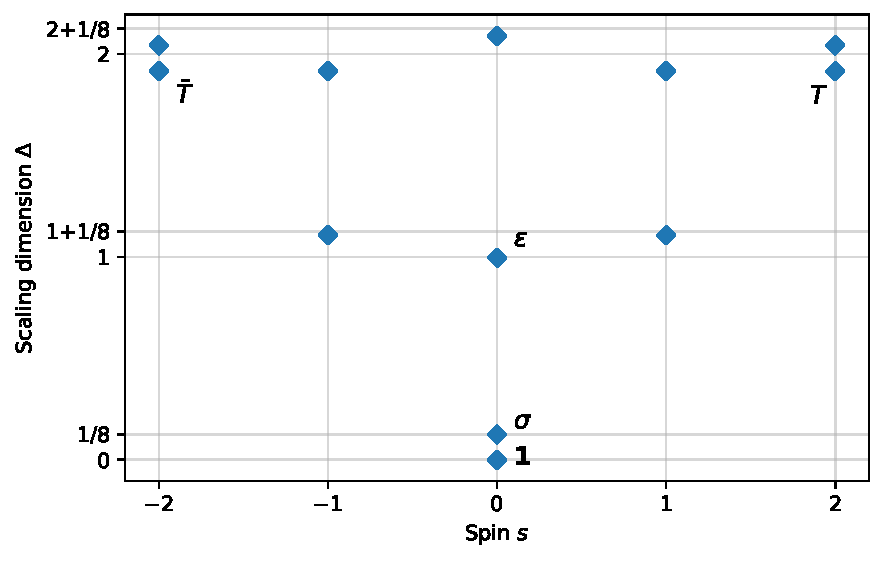
\includegraphics[width=0.7\textwidth]{images/fibonacci/ising-spectrum.pdf}
  \caption[Ising 模型的能谱]{Ising 模型的能谱,对应于 $n\to\infty$ 圆柱转移矩阵。其中初级场及能动量张量使用 CFT 中的相应算符来标记。}
  \label{fig:ising-spectrum}
\end{figure}

除了直接考察能谱数据,我们还可以通过分析能动量张量的两点关联函数来检验其正确性,它们可以使用 iTEBD 算法来计算(见 \ref{subsec:mps-time-evolution} 小节)。首先,我们使用 $A$ 张量来构建一个无限一维链 (iMPS),并将其转化为正则形式。接下来,我们通过对 iMPS 进行虚时演化来计算配分函数。再把 $T$ 插入配分函数中,即可计算得到关联函数,其结果如图~\ref{fig:ising-correlation-functions} 所示。可以发现 $T$ 的两点关联函数存在幂律行为,并且拟合得到的标度维数与表~\ref{tab:ising-spectrum} 中的能谱数据大致相符。

\begin{figure}[ht]
  \centering
  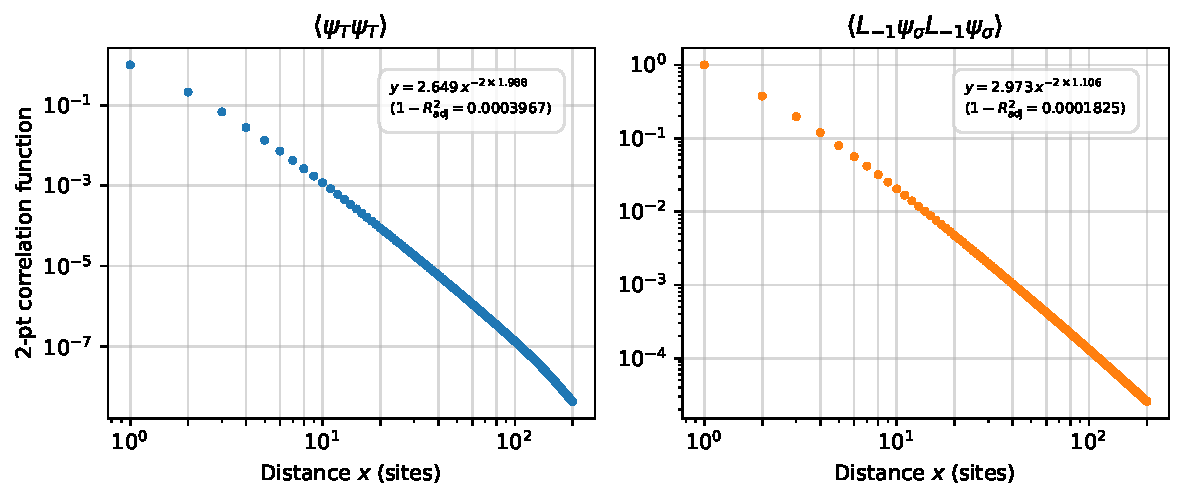
\includegraphics[width=0.9\textwidth]{images/fibonacci/ising-correlation-function.pdf}
  \caption[Ising 模型中的两点关联函数]{Ising 模型中能动量张量 $T$(左图)和 $L_{-1}\phi_\sigma$(右图)的两点关联函数。为了避免计算本征值时有限尺寸效应导致的误差(影响 $x$ 较小的区间),以及 iTEBD 算法中的长程累积误差(影响 $x$ 较大的区间),我们只取 $x=10$ 到 100 区间的数据来拟合幂律公式 $y=Ax^{-2\Delta}$,此时分别得到 $\Delta=1.988$ 和 1.106。它们与 Ising 能谱的理论结果($\Delta=2$ 和 $1+1/8$)基本相符。}
  \label{fig:ising-correlation-functions}
\end{figure}

\subsection{Virasoro 算符}
\label{subsec:ising-virasoro-operator}

注意到此时 $T$ 和 $\bar{T}$ 的形状和 $A^{(1)}$ 是相同的,我们便可以按照图~\ref{fig:virasoro-construction} 的方法来构造 Virasoro 算符。这里我们仍然选取 $N=8$ 的圆柱,但组成它的张量单元都是经过粗粒近似的 $A^{(1)}$,其连接维数 $\chi=4$。

\begin{figure}[ht]
  \centering
  \includegraphics[width=0.4\textwidth]{images/temp/virasoro-operator.pdf}
  \caption[Virasoro 算符作用在本征态上]{Virasoro 算符(或 Kac--Moody 算符)作用在本征态上。}
  \label{fig:virasoro-operator}
\end{figure}

为了检验这一方法的正确性,我们把得到的 Virasoro 算符 $L_n$ 和 $\bar{L}_n$ 进一步作用在 $N=8$、$\chi=4$ 圆柱的本征态 $\ket*{\phi_\alpha}$ 上(如图~\ref{fig:virasoro-operator} 所示)。在 CFT 中,Virasoro 算符起到升降算符的作用,使得
\begin{equation}
  L_n         \ket{\Delta_\alpha, s_\alpha} \propto \ket{\Delta_\alpha-n, s_\alpha-n}, \quad
  L_{\bar{n}} \ket{\Delta_\alpha, s_\alpha} \propto \ket{\Delta_\alpha-n, s_\alpha+n}.
\end{equation}
因此只需考察矩阵元 $\langle\phi_\beta|L_n|\phi_\alpha\rangle$ 的值,即可判断 $L_n$ 和 $\bar{L}_n$ 是否能将 $\ket*{\phi_\alpha}$ 映射到相应的态上。我们的计算结果显示,在 Ising 模型中,对于 $N=8$、$\chi=4$ 圆柱的本征态,近似有
\begin{equation}
  \frac{\lVert \langle\phi_\beta|L_n|\phi_\alpha\rangle \rVert}{\lVert \ket*{\phi_\beta} \rVert \cdot \lVert L_n\ket*{\phi_\alpha} \rVert} \gtrsim 0.9, \quad
  n=\pm1, \pm2.
\end{equation}
这说明通过本方法计算得到的格点 Virasoro 算符与 CFT 的理论预言基本是一致的,并且具有比较好的精度。在图~\ref{fig:ising-virasoro} 和 \ref{fig:ising-virasoro-all} 中,我们给出了这些格点 Virasoro 算符作用的示意图。矩阵元的数据可以在文献 \parencite{wang2022virasoro} 的补充材料中找到。我们观察到,在这些矩阵元中,有一些数据的精度相对较低(与正确值相差 1 到 2 个数量级)。造成这种问题的原因主要是格点模型的有限尺寸效应:一方面,在比较小的圆柱中,CFT 的不同本征态实际上是存在交叠的;另一方面,格点 Virasoro 算符也是通过对有限大小的圆柱进行精确对角化求得的,本身也存在一定误差。

Virasoro 算符的正确性同样可以通过两点关联函数来检验。在图~\ref{fig:ising-correlation-functions} 中,我们考察了 $L_{-1}\phi_\sigma$ 的关联函数,拟合得到的标度维数与理论值 $1+1/8$ 也是基本一致的。

\begin{figure}[ht]
  \centering
  \includegraphics[width=0.7\textwidth]{images/virasoro/ising_spectrum.pdf}
  \caption[Virasoro 算符在 Ising 模型能谱上的作用示意图]{Virasoro 算符 $L_{-1}$ 在 Ising 模型能谱上的作用示意图。能动量张量 $T$ 由 $n=4$、$\chi=4$ 圆柱的本征态得到(左图),由此构造出的 Virasoro 算符 $L_{-1}$ 则作用在 $N=8$、$\chi=4$ 的圆柱上(右图)。更多的例子见图~\ref{fig:ising-virasoro-all}。}
  \label{fig:ising-virasoro}
\end{figure}

\section{例子:Dimer 模型}

接下来我们考虑正方格点上的 dimer 模型\cite{kasteleyn1961statistics,temperley1961dimer,kasteleyn1963dimer}。与 Ising 模型类似,它的配分函数也可以表示为一个二维张量网络,张量单元 $B^{(0)}_{ijkl}$ 中的非零元素为
\begin{equation}
  B^{(0)}_{1111} = B^{(0)}_{2211} = B^{(0)}_{2121} = B^{(0)}_{1212} = B^{(0)}_{2222} = 1, \quad
  B^{(0)}_{1122} = 2.
\end{equation}
在连续极限下,这一模型对应了中心荷 $c=1$ 的自由 Bose 子共形场论\cite{ioffe1989superconductivity,henley1997relaxation,allegra2015exact},其顶点算子 (vertex operator) 具有标度维数和共形自旋
\begin{equation}
  \Delta_{e,m} = e^2 + \frac14 m^2, \quad
  s_{e,m} = em,
\end{equation}
式中 $e$、$m$ 是 dimer 模型 Coulomb 气描述中的电磁荷。

除了 Virasoro 对称性,连续极限下的 dimer 模型还额外具有 Kac--Moody 对称性。由于 Virasoro 生成元的构造方法与 Ising 模型的情况完全一致,这里我们只考察 Kac--Moody 生成元。我们使用 $2\times2$ 个张量单元 $B^{(0)}$ 来构造粗粒近似的张量 $B^{(1)}$,其标度维数 $\chi=4$。对由 $N=4$ 的圆柱(相当于 $N=8$、$\chi=2$ 的圆柱)进行精确对角化可以得到相应的能谱数据,而 $\ket*{\phi_J}$ 和 $\ket*{\phi_{\bar{J}}}$ 就分别对应了 $s=\pm1$ 的两个最低能级。将其变形后可以得到 4 个指标、$\chi=4$ 的张量 $J$ 和 $\bar{J}$,即流算符的近似格点表示。

\begin{figure}[ht]
  \centering
  \includegraphics[width=0.7\textwidth]{images/virasoro/dimer_spectrum.pdf}
  \caption[Kac--Moody 算符在 dimer 模型能谱上的作用示意图]{Kac--Moody 算符 $J_{-1}$ 在 dimer 模型能谱上的作用示意图。近似的流算符 $J$ 由 $n=4$、$\chi=4$ 圆柱的本征态得到(左图),由此构造出的 Kac--Moody 算符 $J_{-1}$ 则作用在 $N=8$、$\chi=4$ 的圆柱上(右图)。其中,符合 CFT 预测的作用使用黑色实线箭头标记,而不相符的则用灰色虚线箭头标记。更多的例子见图~\ref{fig:dimer-kac-moody-all}。}
  \label{fig:dimer-kac-moody}
\end{figure}

同样按照图~\ref{fig:virasoro-construction} 和 \ref{fig:virasoro-operator} 中的方法,我们选取 $N=8$、$\chi=4$ 的圆柱来构造并检验 Kac--Moody 生成元。Kac--Moody 算符满足
\begin{equation}
  J_n         \ket{\Delta_\alpha, s_\alpha} \propto \ket{\Delta_\alpha-n, s_\alpha-n}, \quad
  J_{\bar{n}} \ket{\Delta_\alpha, s_\alpha} \propto \ket{\Delta_\alpha-n, s_\alpha+n}.
\end{equation}
因此通过考察矩阵元 $\langle\phi_\beta|J_n|\phi_\alpha\rangle$ 即可判断 $J_n$ 和 $\bar{J}_n$ 是否能正确起到升降算符的作用。计算结果表明,对于初始态 $\ket{\phi_\alpha}=\ket{\Delta_\alpha,s_\alpha}$,按上述方法构造出的格点 Kac--Moody 算符能够将其映射到正确的后代 $\ket{\phi_\beta}=\ket{\Delta_\beta,s_\beta}$ 上。然而,在这些矩阵元中我们也观察到了一些错误值。相比于 Ising 的情况,dimer 模型中有更严重的限尺寸效应,因而误差也更加显著。这些错误值主要有以下两类:

\begin{enumerate}
  \item 不同 Kac--Moody 后代之间的混淆(主要是 $\ket{s=0,\Delta=0}$ 和 $\ket{s=0,\Delta=1}$ 的后代之间),这可能是由于圆柱的最低本征态并非真实的真空态,而是包含了其他初级场的污染;
  \item 同一组 Kac--Moody 后代中升/降作用的混淆,这表明格点流算符的全纯与反全纯部分很可能没有完全分离。
\end{enumerate}

需要指出的是,这些矩阵元之间的混淆具有一些特定的模式(见文献 \parencite{wang2022virasoro} 补充材料中的数据),这说明计算所得的基态是真实的真空态与一些较低能级简并态的混合,而且混合关系是固定的。此外我们还可以观察到,相比那些不能通过 Kac--Moody 代数从某些初级场生成的能级,矩阵元之间的差异仍有 5--6 个数量级。因而这表明我们的构造方案仍染有效,并且原则上也可以将这些本征态分离开来(可能需要使用更大的圆柱以减小有限尺寸效应的影响)。

\section{例子:Fibonacci 模型}

在很大程度上,Ising 模型具有一定的特殊性,例如它受有限尺寸效应的影响较小。对于更一般的模型,无论是计算与确定圆柱本征态,还是构造对应的 Virasoro 算符,都较为困难。本小节我们将考察 $\mathbb{Z}_3$ parafermion CFT,它可以通过为 Fibonacci 弦网模型添加适当的边界条件而得到。

\subsection{转移矩阵}

Fibonacci 弦网模型定义在六边形网格上,包含 $\1$ 和 $\tau$ 两种简单对象,对应的三角形张量单元已经在 \ref{subsec:strange-correlator-fib} 小节中给出:
\begin{equation}
    \Triangle \tau\tau\tau\tau\tau\tau
  = \varphi^{\frac14} \bigl[ F^{\tau\tau\tau}_\tau \bigr]_{\tau\tau} = -\varphi^{-\frac34}, \quad
    \Triangle \tau\tau\tau\1\tau\tau
  = \varphi^{\frac{7}{12}} \bigl[ F^{\tau\tau\tau}_\tau \bigr]_{\tau\1} = \varphi^{\frac{1}{12}}.
  \label{eq:fib-triangles}
\end{equation}
为了沿用前面处理 Ising 模型时的思路,我们首先需要把两个三角张量形拼合成一个正方形:
\begin{equation}
  A_{ijkl} = \tikzinput{fib-square-1} = \tikzinput{fib-square-1}.
  \label{eq:fib-square}
\end{equation}
同样,转移矩阵也是由张量单元 $A$ 构成的:
\begin{equation}
    \tilde{M}_{i_1 i_2 \cdots i_n, \, j_1 j_2 \cdots j_n}
  = \sum_{\substack{i_1, i_2, \ldots, i_n \\ j_1, j_2, \ldots, j_n}}
    \prod_{\alpha=1}^n A_{i_\alpha j_\alpha j_{\alpha+1} i_{\alpha+1}}
  = \tikzinput{fib-cylinder} \, .
\end{equation}
但与正方格点(如二维 Ising 模型)的情况不同,这里 $A_{ijkl}$ 的指标位于四个角,所以在缩并时需要仔细处理各指标的顺序。此外,上述圆柱 $\tilde{M}$ 并不是 Hermitian 的,因此并不能直接构成正确的转移矩阵。如果把 这些圆柱堆叠起来,在最终计算得到的能谱中将会出现额外的相位。我们可以把两个方向相反的圆柱叠加起来,即选取
\begin{equation}
  M = \tilde{M}\tilde{M}^\dagger,
\end{equation}
这时就可以消除相位的影响,得到正确的转移矩阵。

\subsection{CFT 能谱与能动量张量}

在热力学极限下,Fibonacci 弦网模型(也即中心荷 $c=4/5$ 的 hard-hexagon 模型)将会收敛到 $\mathbb{Z}_3$ parafermion CFT,但并非所有的拓扑缺陷在格点近似中都存在对应的矩阵乘积算符 (MPO) 表示\cite{vanhove2018mapping}。我们并不需要考虑拓扑缺陷,而这种“空”的环面配分函数可以通过取大小为 $n=3k$ 的圆柱得到。相应地,平移算符也需要改为使用把格点平移 3 个单位的 $P^3$。

随着圆柱尺寸 $n$ 的增加,计算中内存消耗是指数级增长的。为了能够处理较大的圆柱,我们这里采用了矩阵无关 (matrix-free) 的线性算符 (linear operator) 方法,即不再显式地构造转移矩阵 $M$,而是计算 $M$ 作用在某个向量上的结果。如图~\ref{fig:fib-linear-operator} 所示,由于 $M$ 是通过张量单元 $A_{ijkl}$ 构造而成的,矩阵乘法 $M\cdot v$ 可利用多次张量缩并来实现。而平移算符则可以通过对数组元素的重新排列来获得。对于大小为 $n$ 的圆柱,线性算符方法可将内存消耗由 $\mathcal{O}(\chi^{2n})$ 降低到 $\mathcal{O}(\chi^n)$。对于 Fibonacci 模型的情况,在典型配置的服务器上最大可以计算到约 $n\simeq30$ 的情形。

\begin{figure}[ht]
  \tikzinput{fib-linear-operator}
  \caption[利用线性算符方法实现矩阵乘法]{对于 Fibonacci 弦网模型,利用线性算符方法实现矩阵乘法 $M\cdot v$。}
  \label{fig:fib-linear-operator}
\end{figure}

计算得到的能谱数据列在表~\ref{tab:fib-spectrum} 中。由于 Fibonacci 模型中有限尺寸效应较为显著,只有 $n\gtrsim20$ 的圆柱本征值才能给出相对准确的结果。对于较小的圆柱体,一些激发态可能甚至不会出现在能谱中。原则上,将计算结果与标度维数和自旋的理论值进行对比,即可确定对应能级的本征态,例如能动量张量对应的 $\ket*{\phi_T}$。但由于有限尺寸效应,不仅本征值与其理论结果相差甚远,而且还普遍存在能级交错的现象——当圆柱较小时,某些在热力学极限下本应位于较高激发态的能级反而会拥有较小的本征值,这样就很难与其他能级区分开来。

为了在有限尺寸下也能区分不同的本征态,首先我们假设标度维数 $\Delta$ 将大致按照
\begin{equation}
  \Delta = A + \frac{B}{n}
\end{equation}
的形式趋近于其热力学极限值\cite{schuler2016universal},然后我们在能谱中选择相应的数据以使拟合结果最优(即挑选出最接近拟合曲线的数据点,见图~\ref{fig:fib-fitting})。计算出拟合参数 $A$ 后,令 $n\to\infty$ 即可得到 $\Delta^\infty$。这些数据列在表~\ref{tab:fib-spectrum} 的“$\infty$”栏中。进一步,我们还根据式~\eqref{eq:scaling-dimension-rescale} 标定了能谱中的本征值,使得 $\Delta_{\1}=0$、$\Delta_T=2$,从而可以更为准确地估计标度维数。这些数据列在了“调整值”一栏,并且绘制在了图~\ref{fig:fib-spectrum} 中。

\begin{figure}[ht]
  \centering
  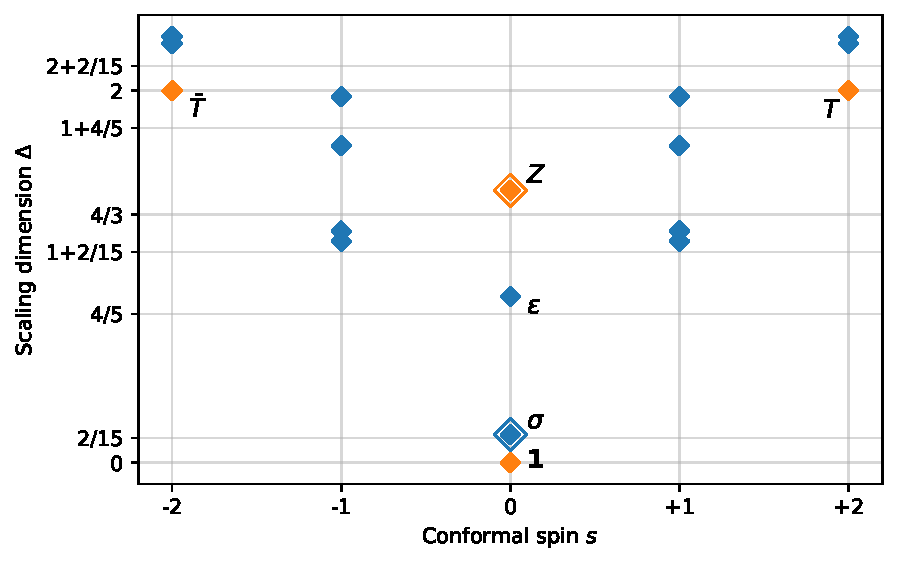
\includegraphics[width=0.7\textwidth]{images/fibonacci/fib-spectrum.pdf}
  \caption[Fibonacci 模型的能谱]{Fibonacci 模型的能谱,对应于 $n\to\infty$ 圆柱转移矩阵。“\tikzinput{fib-spectrum-label}\unskip”表明存在二重简并。图中的本征值进行了缩放处理,以使得 $\Delta_{\1}=0$ 和 $\Delta_T=2$。初级场使用对应的算符来标记,它们的共形维数分别为 $h_{\1}=0$,$h_\sigma=1/15$,$h_\epsilon=2/5$,$h_Z=2/3$,$h_X=7/5$ 以及 $h_Y=3$(与 $X$、$Y$ 对应的态本征值较大,在我们的计算中没有考虑)。CFT 配分函数为 $Z=|\chi_{\1}+\chi_Y|^2+|\chi_\epsilon+\chi_X|^2+2|\chi_\sigma|^2\discretionary{}{}{}+2|\chi_Z|^2$\cite{vanhove2018mapping}。对应于 $|\chi_{\1}+\chi_Y|^2$ 的子空间,其中的本征态用橙色标记。}
  \label{fig:fib-spectrum}
\end{figure}

在拟合中还可以考虑高阶修正项,如
\begin{equation}
  \Delta = A + \frac{B}{n} + \frac{C}{n^2},
\end{equation}
其拟合结果在图~\ref{fig:fib-fitting} 中用虚线标出。高阶项可以给出更好的拟合结果,但由于我们只需要通过这一方法来确定 CFT 中的各能级,因此只需考虑一阶修正项。

\begin{figure}[ht]
  \centering
  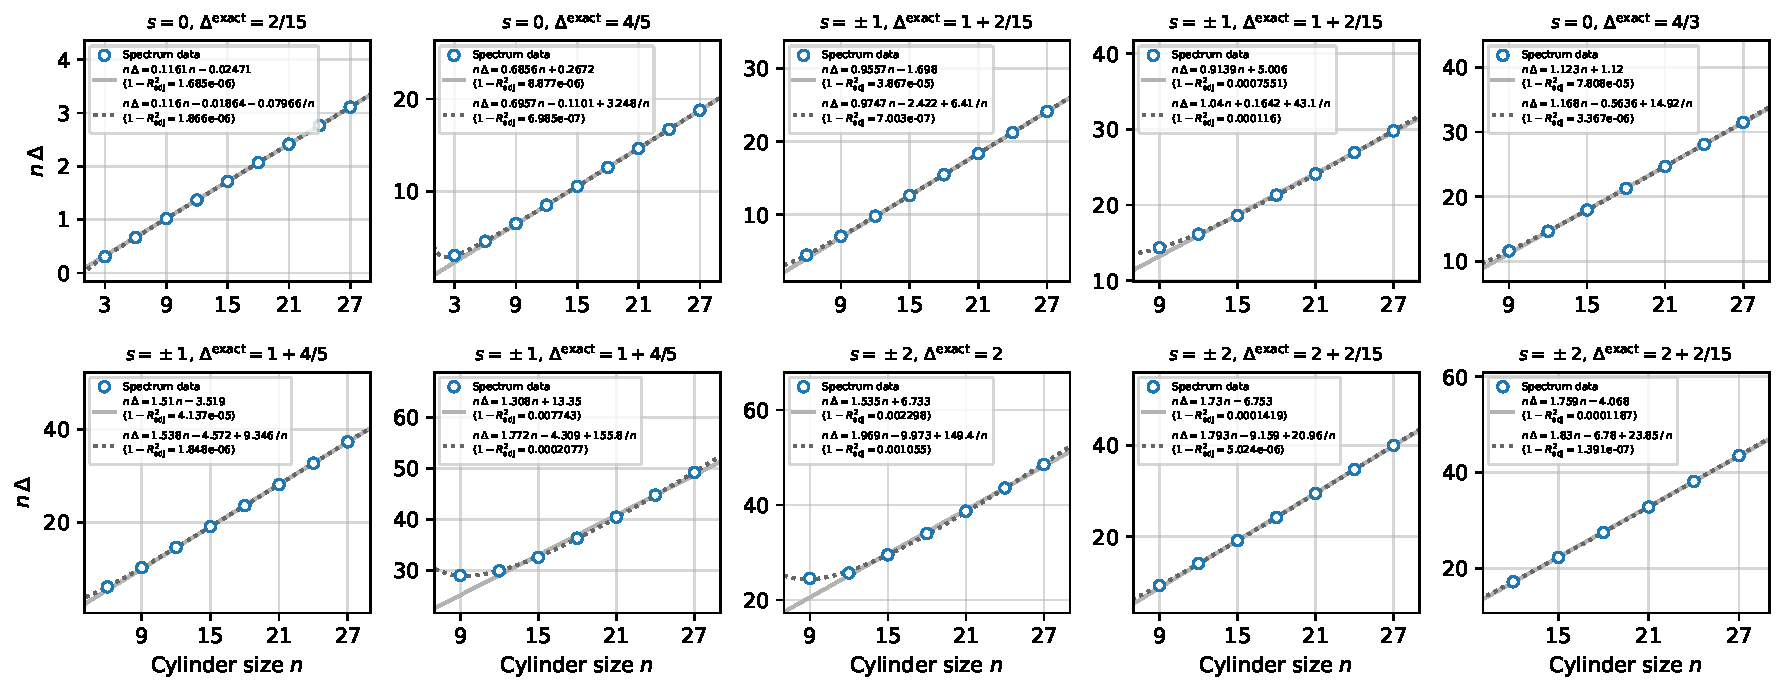
\includegraphics[width=\textwidth]{images/fibonacci/fib-fitting.pdf}
  \caption[Fibonacci 能谱的拟合结果]{Fibonacci 能谱的拟合结果。在拟合 $n\Delta=An+B$ 时,我们仅使用了 $n=12$ 到 27 的圆柱(实线);而在拟合 $n\Delta=An+B+C/n$ 时,我们使用了所有可用的 $n$(虚线)。}
  \label{fig:fib-fitting}
\end{figure}

\subsection{拓扑投影算符}
\label{subsec:topological-projectors}

然而,当太多能级混杂在一起时,上述的拟合方法也无法保证能够将各能级区分开来。例如,当两个能级的自旋相同、标度维数又很接近时,仅从拟合优度并不能分辨。为此,我们需要利用\emph{拓扑投影算符} (topological projectors)\cite{bultinck2017anyons,williamson2017symmetry,aasen2020topological},它可以将转移矩阵投影到对应于特定拓扑荷 (topological charge) 的子空间。拓扑荷与格点模型的尺寸是无关的,因此在热力学极限下趋于能动量张量的本征态,即使在有限大小的系统中也仍然会保持在同一个分区 (sector) ,即包含了真空态的平凡分区。它们在特定的投影算符作用之下可以保留在能谱中,而其他态则会被移除(即投影到零值)。

拓扑投影算符的构造与 \emph{Ocneanu 管状代数} (Ocneanu's tube algebra)\cite{evans1995ocneanu,evans1998quantum}有关。拓扑序模型中的每种任意子都对应着 CFT 中的一个拓扑分区,换而言之 CFT 中的初级场及其后代组成的“家族” (family) 可按照对应的任意子类型进行分类。拓扑序中的弦算符则可作为投影算符,将转移矩阵投影到包含相应拓扑分区的子空间上。因为我们这里的工作主要关注能动量张量,而能动量张量与真空态属于同一分区,所以只需构造与任意子 $\1$ 相对应的弦算符。

弦算符的一般形式可由 MPO 来描述,称为\emph{幂等元} (idempotent)\cite{bultinck2017anyons,williamson2017symmetry,vanhove2018mapping,lootens2019cardy,aasen2020topological}。构成这些 MPO 的矩阵单元为
\begin{equation}
  \begin{aligned}
       \tikzinput{idempotents-mpo-1}
    &= (d_\alpha d_\beta d_\gamma d_\delta)^{\frac14} G^{\beta i\gamma}_{j\alpha\delta}, \\
       \tikzinput{idempotents-mpo-2}
    &= (d_\alpha d_\beta d_\gamma d_\delta d_i d_j d_k)^{\frac14}
       G^{k\beta\delta}_{ij\alpha} G^{i\gamma\beta}_{kj\delta},
  \end{aligned}
\end{equation}
其中 $G$ 可通过对四面体张量($F$ 符号)进行归一化和对称化得到:
\begin{equation}
    G^{abc}_{ijk}
  = \frac{1}{\sqrt{d_j d_c}} \bigl[ F^{aik}_b \bigr]_{jc}
  = \frac{1}{\sqrt{d_a d_b d_c d_i d_j d_k}} \, \Tetrahedron jibcka.
\end{equation}
对于大小为 $n$ 的圆柱转移矩阵,管状代数的基可由 $n-1$ 个橙色张量与一个红色张量首尾相连得到:
\begin{equation}
  \mathcal{T}_{ab}^c = \tikzinput{tube-algebra-basis}.
\end{equation}
注意图中省略了辅助指标,它们需要被正常缩并掉。

幂等元的一般形式可表示为这些基的线性组合。在 Fibonacci 模型中,对应于 $\1$ 的弦算符幂等元为\cite{bultinck2017anyons}
\begin{equation}
  \mathcal{P}_1 = \frac{1}{\sqrt5}
  \left( \frac{1}{\phi} \mathcal{T}^{\1}_{\1\1} + \sqrt{\phi} \mathcal{T}^\tau_{\tau\1} \right).
\end{equation}
它可以与转移矩阵、平移算符相连,再进行对角化便可得到只含真空态、能动量张量等的子能谱。这样,即使是在有限尺寸下,依然可以严格地找到能动量张量对应的本征态。我们在表~\ref{tab:fib-spectrum} 和图~\ref{fig:fib-spectrum} 中都对这些态做了高亮。

\subsection{Virasoro 算符}

接下来我们按照 \ref{sec:virasoro-operators} 节中介绍的方法来构造 Virasoro 算符。考虑到 Fibonacci 模型要求圆柱大小 $n=3k$,此时由对角化求得的能动量张量 $T$ 和 $\bar{T}$ 并不能像 Ising 模型的情况一样直接插回圆柱。因此,我们需要首先把 $T$ 和 $\bar{T}$ 变形为三角形,再用式~\eqref{eq:fib-triangles} 中的三角形张量单元补成正方形,这与式~\eqref{eq:fib-square} 是类似的:
\begin{equation}
  \tikzinput{fib-padded-tensor-1} = \tikzinput{fib-padded-tensor-2} \to \tikzinput{fib-padded-tensor-3}.
\end{equation}
注意在缩并时只有角上的自由度需要考虑。圆柱中的其他张量也可以用类似的方式构造,但方便起见,也可以等价地用 $k\times k$ 个式~\eqref{eq:fib-square} 中的正方形缩并得到。

计算中我们用 $n=18$ 的圆柱来计算本征态,并得到对应的能动量张量。之后,将其变形并补全成正方形张量,此时连接维数 $\chi=2^{n/3}$。我们同样按照图~\ref{fig:virasoro-construction} 的方式构造 Virasoro 算符。尽管原则上圆柱的大小 $N$ 可以取任意值,但由于内存的限制,这里最大只能取到 $N=3$。检验 Virasoro 算符正确性的方法与 \ref{subsec:ising-virasoro-operator} 小节相同,也是检查 $L_n$ 和 $\bar{L}_n$ 是否能将圆柱本征态 $\ket*{\phi_\alpha}$ 正确地升高或降低到对应能级。在图~\ref{fig:fib-virasoro} 和 \ref{fig:fib-virasoro-all} 中,我们给出了这些格点 Virasoro 算符作用的示意图。矩阵元的数据则可在文献 \parencite{zeng2023virasoro} 的补充材料中找到。

\begin{figure}[ht]
  \centering
  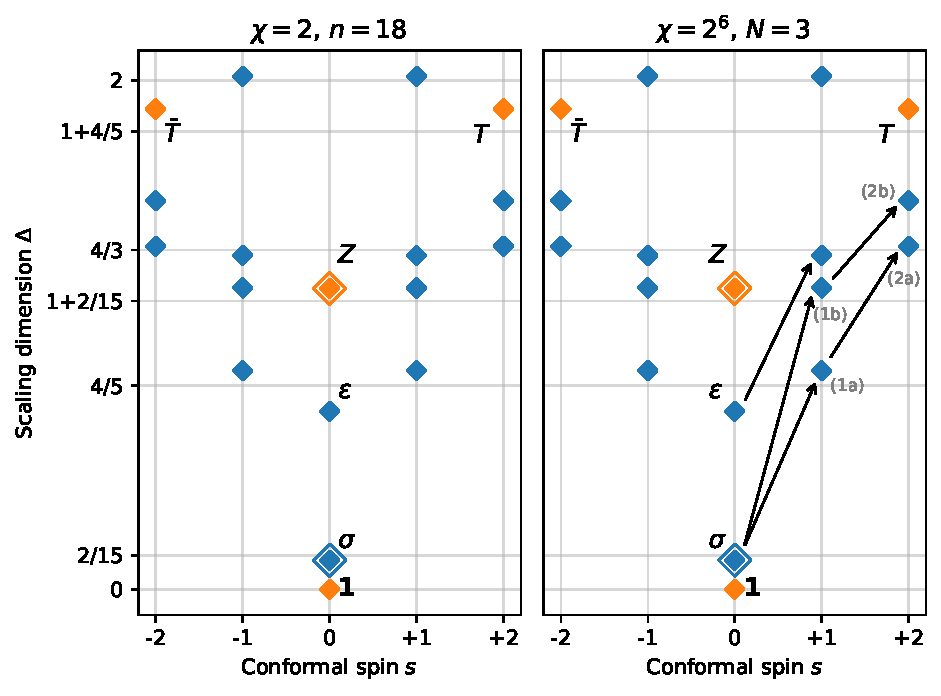
\includegraphics[width=0.7\textwidth]{images/fibonacci/fib-virasoro.pdf}
  \caption[Virasoro 算符在 Fibonacci 模型能谱上的作用示意图]{Virasoro 算符 $L_{-1}$ 在 Fibonacci 模型能谱上的作用示意图。能动量张量 $T$ 由 $n=18$、$\chi=2$ 圆柱的本征态得到(左图),由此构造出的 Virasoro 算符 $L_{-1}$ 则作用在 $N=3$、$\chi=2^{n/3}$ 的圆柱上(右图)。标记为 (1a)/(1b) 和 (2a)/(2b) 的两组本征态在 CFT 极限下应当是简并的,但由于有限尺寸效应,它们的标度维数并不相同(可对比图~\ref{fig:fib-spectrum})。更多的例子见图~\ref{fig:fib-virasoro-all}。}
  \label{fig:fib-virasoro}
\end{figure}

\section{本章小结}
